%----------------------------------------------------------------------------------------
%	PACKAGES AND OTHER DOCUMENT CONFIGURATIONS
%----------------------------------------------------------------------------------------
%----------------------------------------------
\documentclass[final]{beamer}
\usepackage{mwe} %added this to use other package
\usepackage[scale=1.24]{beamerposter} % Use the beamerposter package for laying out the poster

\usetheme{confposter} % Use the confposter theme supplied with this template

\setbeamercolor{block title}{fg=jblue,bg=white} % Colors of the block titles
\setbeamercolor{block body}{fg=black,bg=white} % Colors of the body of blocks
\setbeamercolor{block alerted title}{fg=white,bg=dblue!70} % Colors of the highlighted block titles
\setbeamercolor{block alerted body}{fg=black,bg=dblue!10} % Colors of the body of highlighted blocks
% Many more colors are available for use in beamerthemeconfposter.sty

%-----------------------------------------------------------
% Define the column widths and overall poster size
% To set effective sepwid, onecolwid and twocolwid values, first choose how many columns you want and how much separation you want between columns
% In this template, the separation width chosen is 0.024 of the paper width and a 4-column layout
% onecolwid should therefore be (1-(# of columns+1)*sepwid)/# of columns e.g. (1-(4+1)*0.024)/4 = 0.22
% Set twocolwid to be (2*onecolwid)+sepwid = 0.464
% Set threecolwid to be (3*onecolwid)+2*sepwid = 0.708

\newlength{\sepwid}
\newlength{\onecolwid}
\newlength{\twocolwid}
\newlength{\threecolwid}
\setlength{\paperwidth}{48in} % A0 width: 46.8in
\setlength{\paperheight}{36in} % A0 height: 33.1in
\setlength{\sepwid}{0.024\paperwidth} % Separation width (white space) between columns
\setlength{\onecolwid}{0.22\paperwidth} % Width of one column
\setlength{\twocolwid}{0.464\paperwidth} % Width of two columns
\setlength{\threecolwid}{0.708\paperwidth} % Width of three columns
\setlength{\topmargin}{-0.5in} % Reduce the top margin size
%-----------------------------------------------------------

\usepackage{graphicx}  % Required for including images

\usepackage{booktabs} % Top and bottom rules for tables

%----------------------------------------------------------------------------------------
%	TITLE SECTION 
%----------------------------------------------------------------------------------------

\title{Multi-Package UAV Delivery System} % Poster title
%\subsection{Capstone project}

\author{Daniel Lavell, Brandon Luu, Yegeta Zeleke} % Author(s)

\institute{University of California, Santa Cruz} % Institution(s)

%----------------------------------------------------------------------------------------

\begin{document}
\setbeamertemplate{headline}{
 \leavevmode
  \begin{columns}
   \begin{column}{.2\linewidth}
   
\includegraphics[width=0.9\linewidth]{./images/baskin-logo-normal.jpg}
   \end{column}
   \begin{column}{.6\linewidth}
    \vskip1cm
    \centering
    \usebeamercolor{title in headline}{\color{jblue}\Huge{\textbf{\inserttitle}}\\[0.5ex]}
    \usebeamercolor{author in headline}{\color{fg}\Large{\insertauthor}\\[1ex]}
    \usebeamercolor{institute in headline}{\color{fg}\large{\insertinstitute}\\[1ex]}
    \vskip1cm
   \end{column}
   \begin{column}{.2\linewidth}
    
\includegraphics[width=0.9\linewidth]{./images/hsl-logo.png}
   \end{column}
   \vspace{1cm}
  \end{columns}
 \vspace{0.5in}
 %\hspace{0.5in}\begin{beamercolorbox}[wd=47in,colsep=0.15cm]{cboxb}\end{beamercolorbox}
 \vspace{0.1in}
}
%--------------------------------------------------------------------------------------------

\addtobeamertemplate{block end}{}{\vspace*{2ex}} % White space under blocks
\addtobeamertemplate{block alerted end}{}{\vspace*{2ex}} % White space under highlighted (alert) blocks

\setlength{\belowcaptionskip}{2ex} % White space under figures
\setlength\belowdisplayshortskip{2ex} % White space under equations

\begin{frame}[t] % The whole poster is enclosed in one beamer frame

\begin{columns}[t] % The whole poster consists of three major columns, the second of which is split into two columns twice - the [t] option aligns each column's content to the top

\begin{column}{\sepwid}\end{column} % Empty spacer column

\begin{column}{\onecolwid} % The first column


%----------------------------------------------------------------------------------------
%	Abstract
%----------------------------------------------------------------------------------------
\begin{block}{Abstract}
{\small\textbf{\textit{For a few years now, delivery companies have been developing a variety of package-delivery systems using drones. Such technologies will most likely be integrated and implemented into fully functioning autonomous Unmanned Aerial Systems (UAS) in the near future. However, the lack of studies on the effect of such a delivery system on the current National Airspace (NAS) traffic is unstudied.  Moreover, storage and performance requirements to implement a fully autonomous delivery system have not yet been quantified. In this project we implemented a test bench to that uses terrain, building, and population data to build an environment in which a package delivery scenario may be run using quadcopters. We showed that how number of vehicle per warehouse, how soon the warehouse guarantee the package to be delivered, and on board storage required to run the system.} }

%This statement requires citation \cite{Smith:2012qr}.
\par}

\end{block}



\begin{figure}
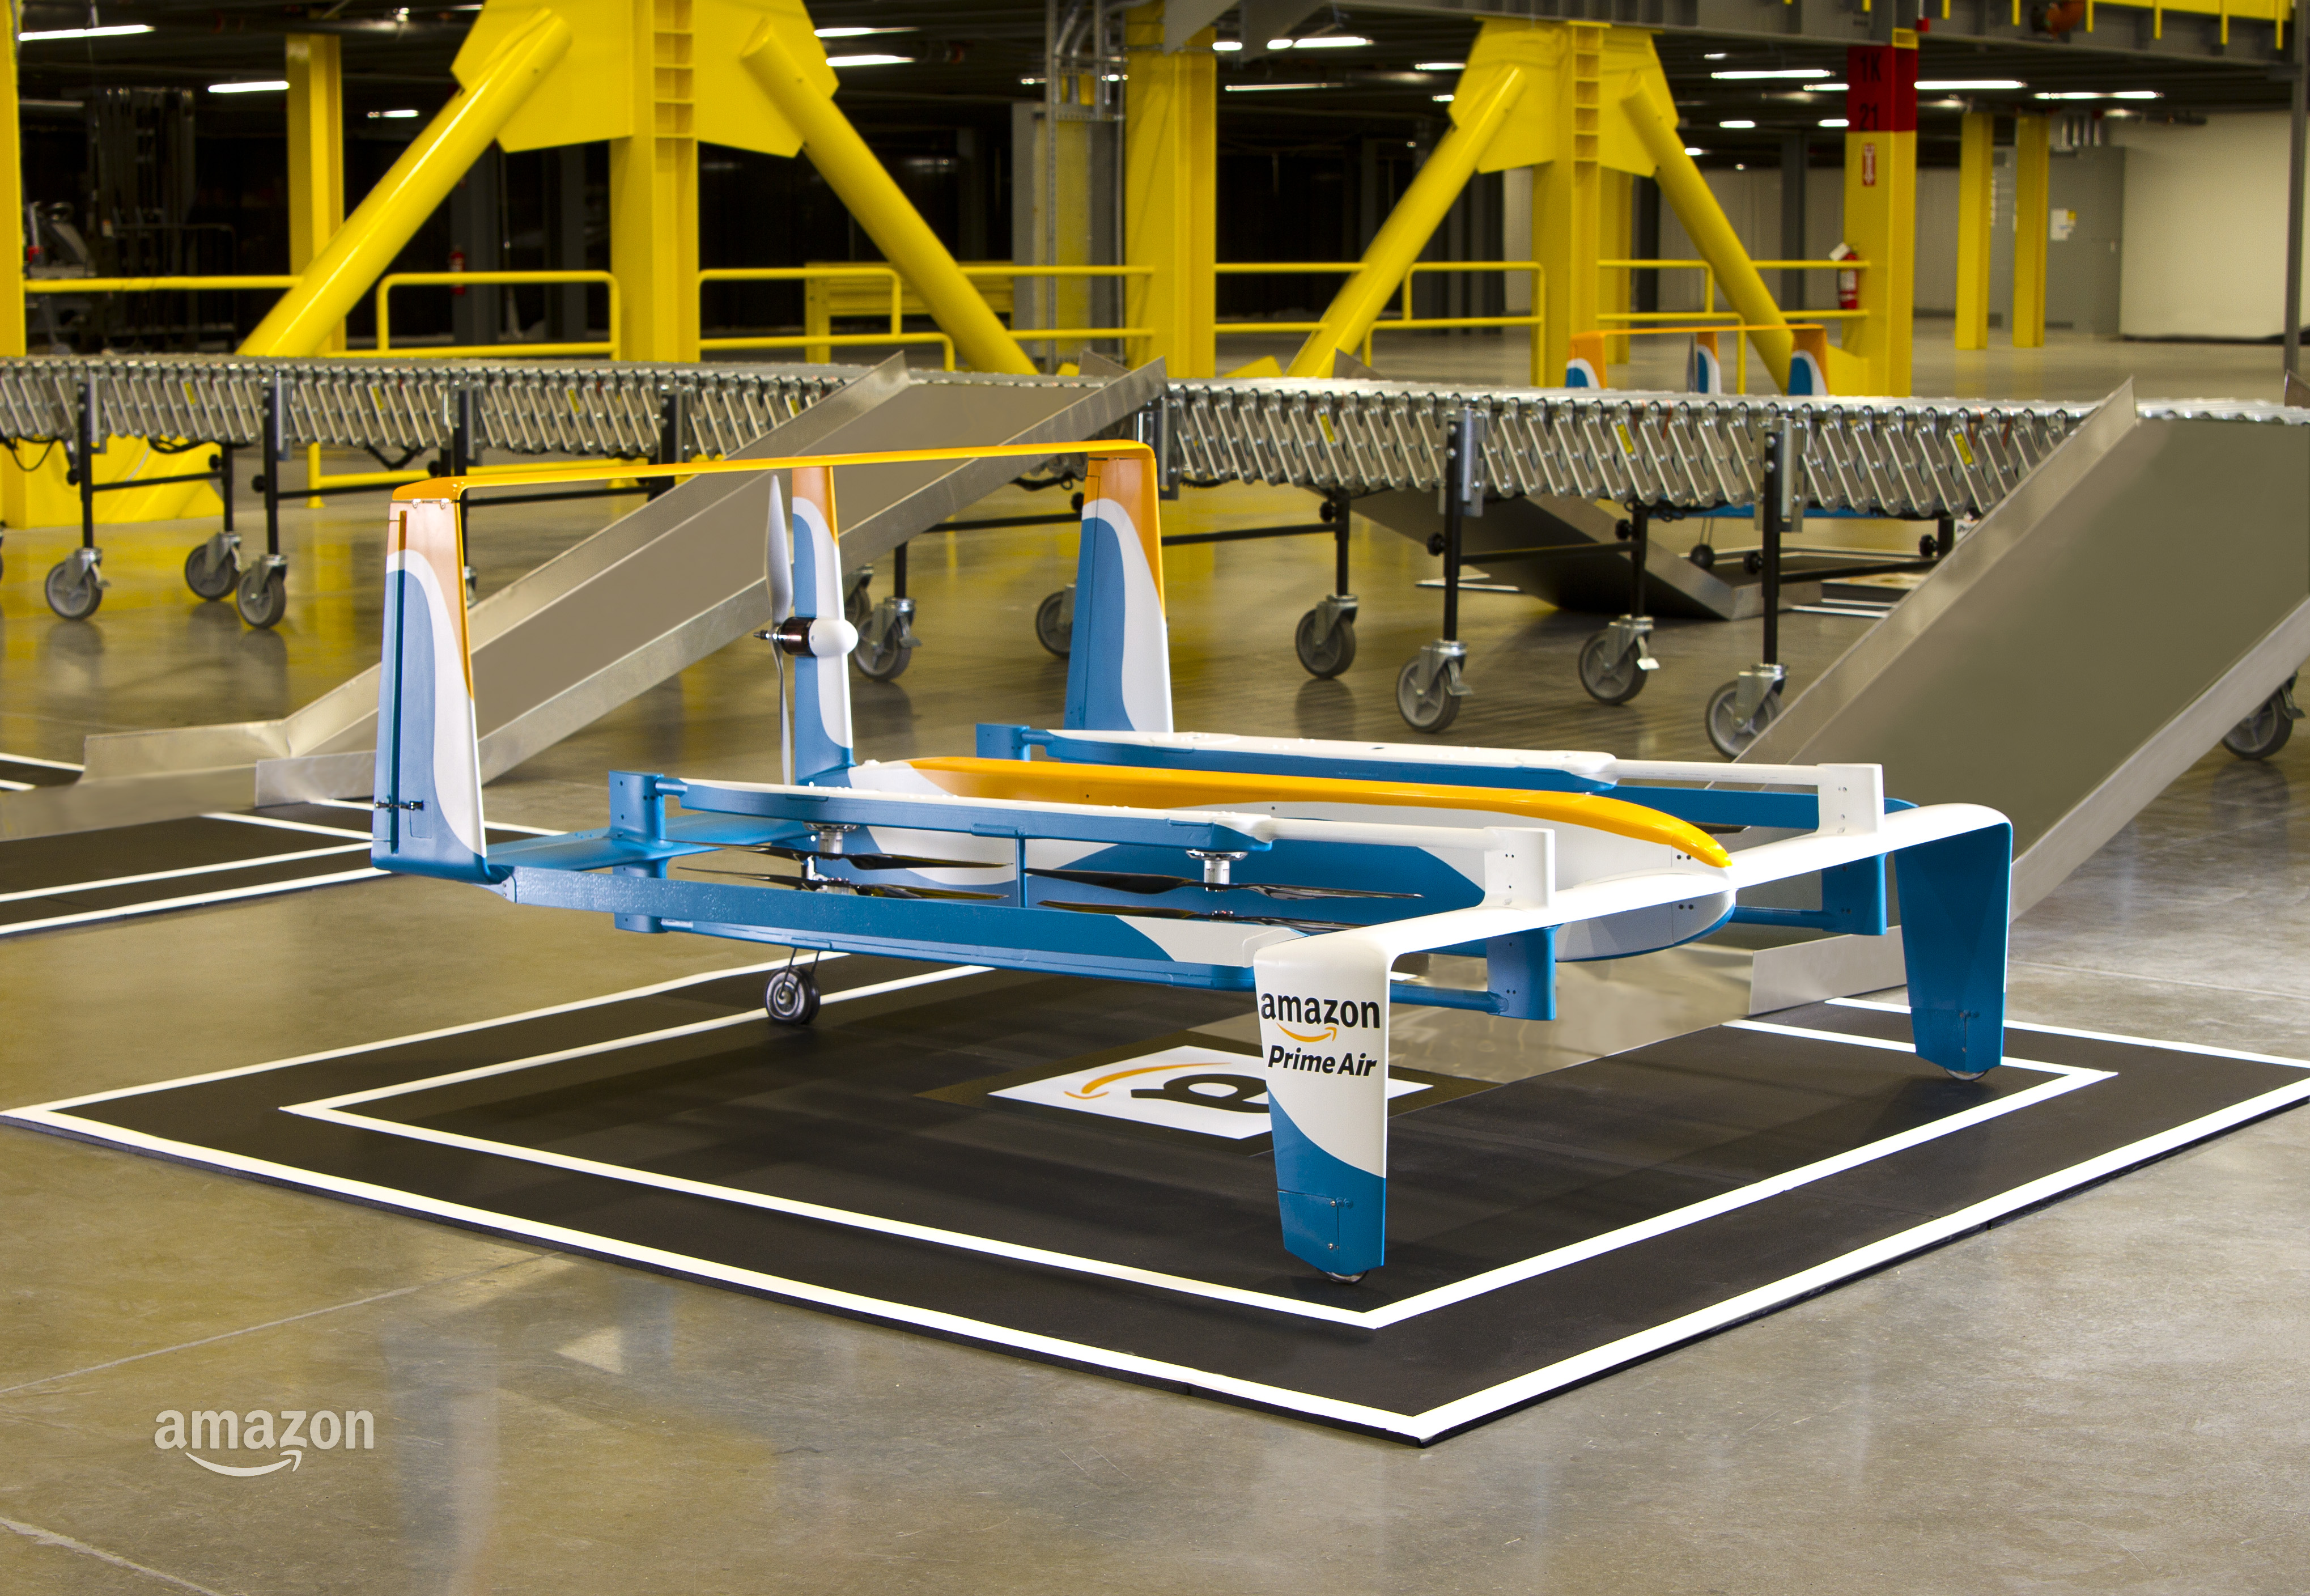
\includegraphics[width=0.8\linewidth]{images/prime-air.jpg}
\caption{Amazon Prime Air Vehicle}
\end{figure}


%----------------------------------------------------------------------------------------
%	INTRODUCTION
%----------------------------------------------------------------------------------------

\begin{block}{Introduction}

{\smallWith growing interest to improve efficiency of package delivery, some companies, such as Amazon, Walmart, and Google, are strongly considering the use of UAV as carriers for the packages. In terms of the NAS, the traffic this would induce has been mostly unstudied. The Federal Aviation Administration (FAA) wants to regulate the air traffic in the NAS in the interest of the people. The companies trying to implement this delivery service want to maximize throughput while meeting time constraints. We propose a solution that meets the requirements of both the FAA and prospective companies using a multiple package per vehicle delivery scheme.
\par}

\end{block}

%------------------------------------------------

%----------------------------------------------------------------------------------------

\end{column} % End of the first column

\begin{column}{\sepwid}\end{column} % Empty spacer column

\begin{column}{\twocolwid} % Begin a column which is two columns wide (column 2)

\begin{columns}[t,totalwidth=\twocolwid] % Split up the two columns wide column

\begin{column}{\onecolwid}\vspace{-.6in} % The first column within column 2 (column 2.1)

%----------------------------------------------------------------------------------------
%	Approach
%----------------------------------------------------------------------------------------

\begin{block}{Approach}
{\small\justify
\begin{enumerate}
\item{Data Collection - In order to simulate a more realistic simulation environment we collected terrain, population, Walmart, and K-12 schools from San Jose. The data was provided from the United States Geological Survey (USGS), United States Census Bureau, Walmart.com, and Schooldigger.com, respectively.}\\

\vspace{7mm}

\item{Initial Framework - The structure of the simulation focused around which warehouses were chosen to have a delivery fleet. Elevation and obstacles around these warehouses are compiled before the simulation runs.}

\vspace{7mm}

\item{Single Package Delivery - UAS vehicles reponded to one package request at a time traversing to the destination and following the same path back to the warehouse.}

\vspace{7mm}

\item{Multiple Package Delivery - After being assigned the first package to deliver, the vehicle waits on the ground until a nearby second package is requested or until there is no more time to wait before missing the time constraint.}

\vspace{7mm}

\item{Analysis - To assess the feasibility of a multiple package per vehicle delivery system, we ran the simulation using both the single and multiple package per vehicle approach comparing the average flight distance, total number of packages delivered, and so as to compare how the vehicle would perform.}
\end{enumerate}
\par}

\end{block}

%----------------------------------------------------------------------------------------

\end{column} % End of column 2.1

\begin{column}{\onecolwid}\vspace{-.6in} % The second column within column 2 (column 2.2)

%----------------------------------------------------------------------------------------
%	System Model
%----------------------------------------------------------------------------------------

\begin{block}{System Model}

{\smallThe vehicle is modeled using a point mass system driven by a controller providing reference points along the trajectory in latitude ($\lambda$) longitude ($\tau$) coordinates pairs. The equations of motion can be described as 


\begin{align}
\dot{\lambda} &= \frac{1}{(R+h)}V_{g}\cos{\textit{X}_{g}} \\
\dot{\tau} &= \frac{1}{(R+h)\cos{\lambda}}V_{g}\sin{\textit{X}_{g}} \\
\dot{h} &= V_{h}
\end{align}

\vspace{5mm}
where $R$ is Earth's radius, $V_{g}$ is the ground speed, $V_{h}$ is the climb rate, $\textit{X}_{g}$ is the tracking angle, and $h$ is the altitude.

\vspace{10mm}

\begin{figure}
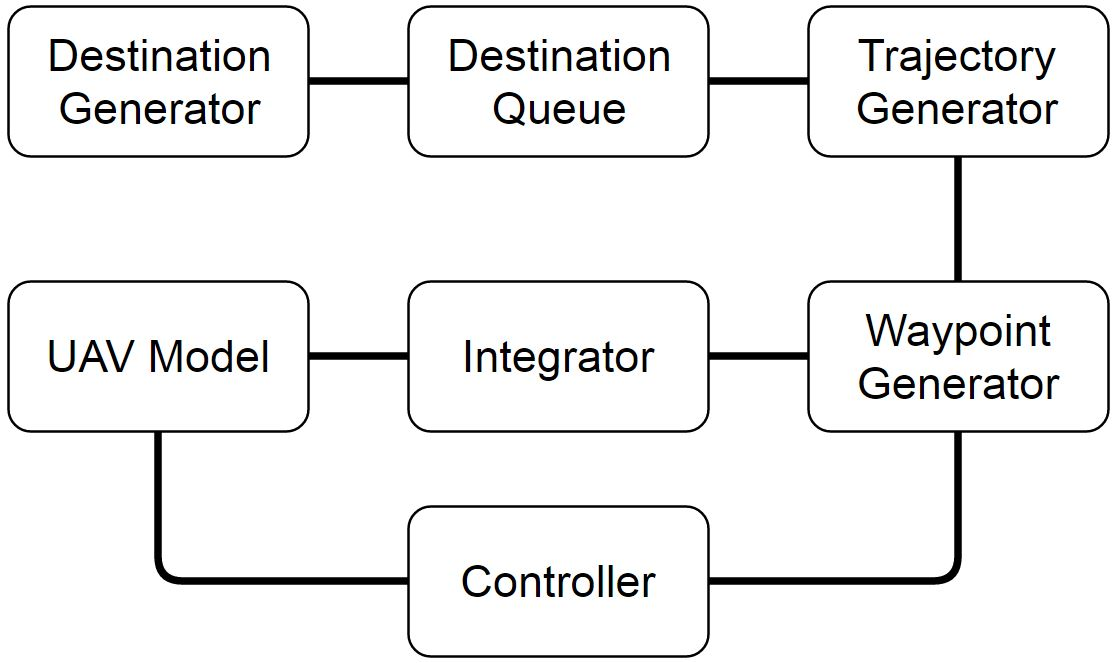
\includegraphics[width=1\linewidth]{images/TopLevelDesign.JPG}
\caption{Simulation Flow Chart}
\end{figure}


\par}

\begin{figure}
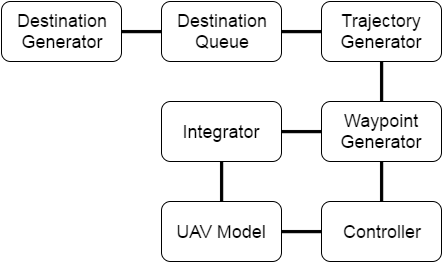
\includegraphics[width=1\linewidth]{images/TopLevelDesign.png}
%\caption{Figure caption}
\end{figure}

\end{block}

%----------------------------------------------------------------------------------------

%%----------------------------------------------------------------------------------------
%%	Analysis
%%----------------------------------------------------------------------------------------
%
%\begin{block}{Analysis}
%
%\textbf{Analysis of the project.....Honestly I don't even know what goes here} \textit{may be some bs?} 


%
%\end{block}
%

%----------------------------------------------------------------------------------------

\end{column} % End of column 2.2

\end{columns} % End of the split of column 2 - any content after this will now take up 2 columns width

%----------------------------------------------------------------------------------------
%	 Overview
%----------------------------------------------------------------------------------------

%\begin{alertblock}{OverView}

{\small\textbf{OverView info goes here}

\par}

\begin{figure}
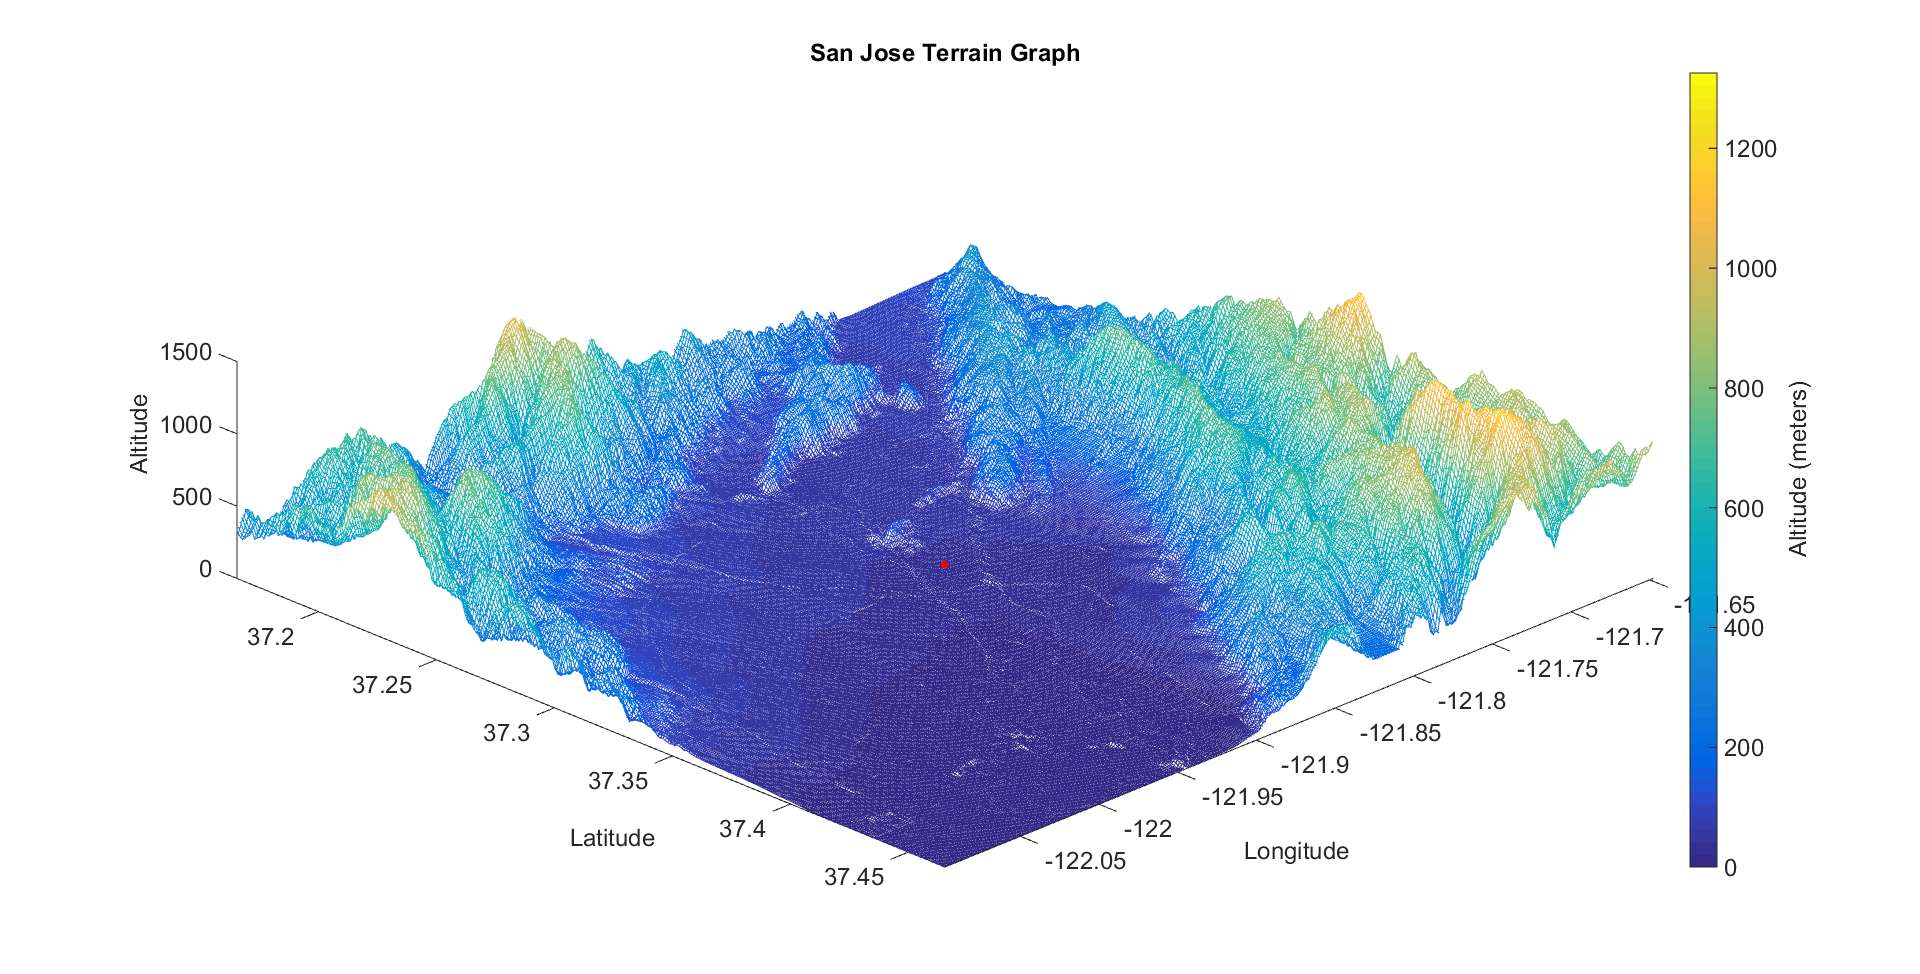
\includegraphics[width=1\linewidth]{images/terrain-side.png}
\caption{Figure caption}
\end{figure}

%\end{alertblock} 

%----------------------------------------------------------------------------------------

%\begin{columns}[t,totalwidth=\twocolwid] % Split up the two columns wide column again

%\begin{column}{\onecolwid} % The first column within column 2 (column 2.1)


%\end{column} % End of column 2.1

%\begin{column}{\onecolwid} % The second column within column 2 (column 2.2)


%\end{column} % End of column 2.2

%\end{columns} % End of the split of column 2

\end{column} % End of the second column

\begin{column}{\sepwid}\end{column} % Empty spacer column

\begin{column}{\onecolwid} % The third column

%----------------------------------------------------------------------------------------
%	RESULTS
%----------------------------------------------------------------------------------------

\begin{block}{Results}
{\small
For both 8 and 4 hours of simulated delivery time, the multiple package delivery system out performed the single package delivery system in overall performance and cost for the delivery service. 
{\footnotesize
\begin{table}[]
\centering
\caption{Simulation Results - Comparing single and multiple packages per vehicle with a 25 vehicle fleet}
\label{my-label}
\begin{tabular}{|l|l|l|l|}
\hline
\begin{tabular}[c]{@{}l@{}}Packages Per\\ Vehicle\end{tabular} & Simulation Time & \begin{tabular}[c]{@{}l@{}}Average Distance\\ Traveled\end{tabular} & Packages Delivered \\ \hline
One-Package                                                    & 8 Hours         & 120 Km    & 121    \\ \hline
One-Package                                                    & 4 Hours         &  67.07 Km & 77     \\ \hline
Two-Packages                                                   & 8 Hours        & 101 Km     & 127    \\ \hline
Two-Packages                                                    & 4 Hours         &  64.4 Km   & 81     \\ \hline
\end{tabular}
\end{table}
}
\vspace{3mm}

By showing that more packages can be delivered when multiple packages are transported by one vehicle, we prove that it would be more cost efficient for a warehouse to invest in vehicles with larger payload capacity. Our simulations also showed that by using the right logic for which packages are assigned to which vehicle, we can ensure that deliveries are made within the time constraint set by the warehouse. We have proved the multiple package delivery system was successful since we delivered more packages using the same resources while reducing the average distance each vehicle had to traverse.
\par}



\begin{figure}
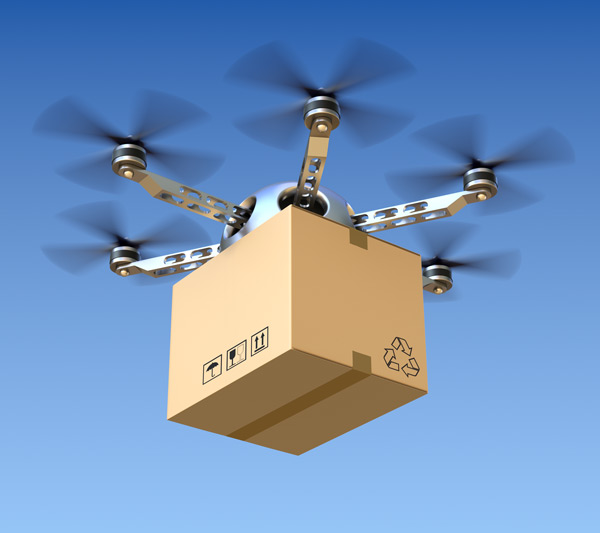
\includegraphics[width=0.8\linewidth]{images/delivery-drone.jpg}
\caption{Figure caption}
\end{figure}

\end{block}

%----------------------------------------------------------------------------------------

%----------------------------------------------------------------------------------------
%	CONCLUSION
%----------------------------------------------------------------------------------------

\begin{block}{Conclusion}
{\smallDue to the highly unstudied nature of this subject, there are many possible future directions that this project can take, some of which include:

\begin{enumerate}
\item{Creating a hardware-in-the-loop testbed, as exemplified in Figure 4.}

\item{Developing a navigation framework necessary to traverse dense urban environments.}

\end{enumerate}
\par}
\end{block}

%----------------------------------------------------------------------------------------

%----------------------------------------------------------------------------------------
%	REFERENCES
%----------------------------------------------------------------------------------------

\begin{block}{References}

\nocite{*} % Insert publications even if they are not cited in the poster
\small{\bibliographystyle{unsrt}
\bibliography{sample}\vspace{0.75in}}

\end{block}

%----------------------------------------------------------------------------------------
%	ACKNOWLEDGEMENTS
%----------------------------------------------------------------------------------------

%\setbeamercolor{block title}{fg=red,bg=white} % Change the block title color

\begin{block}{Acknowledgements}
{\small\small{\rmfamily{We would like to thank Jack Baskin School of Engineering, Professor Ricardo Sanfelice, Professor Patrick Mantey, Eric Cao and all of the friendly members of the Hybrid Systems Lab for all of the support thoughout the course of this project.}} 

\par}

\end{block}


\begin{center}
\begin{tabular}{ccc}

\includegraphics[width=0.4\linewidth]{images/baskin-logo-normal.jpg} & \hfill & 
\includegraphics[width=0.4\linewidth]{images/hsl-logo.png}
\end{tabular}
\end{center}


%----------------------------------------------------------------------------------------
%	CONTACT INFORMATION
%----------------------------------------------------------------------------------------
% COMMENTED OUT!

%\setbeamercolor{block alerted title}{fg=black,bg=norange} % Change the alert block title colors
%\setbeamercolor{block alerted body}{fg=black,bg=white} % Change the alert block body colors

%\begin{alertblock}{Contact Information}
%probably don't need this
%\begin{itemize}
%\item Web: \href{http://www.soe.ucsc.edu}{http://www.soe.ucsc.edu}
%\item Email: \href{mailto:hsl@soe.ucsc.edu}{hsl@soe.ucsc.edu}
%\end{itemize}

%\end{alertblock}


%----------------------------------------------------------------------------------------

\end{column} % End of the third column

\end{columns} % End of all the columns in the poster

\end{frame} % End of the enclosing frame

\end{document}
Status API Training Shop Blog About
© 2016 GitHub, Inc. Terms Privacy Security Contact Help
